\chapter{Impact}
\label{ch:impact}

\section{Introduction}

This chapter details the impact the work described in this thesis has had, including outcomes like artworks that were made by myself and others; recognition, such as exhibitions and awards. 
This also includes an overview of work and research that follows and has been influenced by this research, applications of the research into other domains, and examples of ideas from this thesis being used and put into technologies and practical interfaces. 

\section{\textit{(un)stable equilibrium}}

As a direct outcome of the experiments detailed in Chapter 3, a series of six video artworks titled (un)stable equilibrium 1:1, 1:2, … 1:6 were made by sampling from the paired generative models, in-parallel, using the same latent code (Figure \ref{fig:c7:ue_still}). 
A looping spherical interpolation \citep{white2016sampling} of the two videos was produced, which lasted approximately one hour. 
The interpolations were deliberately designed to be slow to provide a meditative loop seamlessly so that it could be played in a gallery setting without any interruption.

\begin{figure}[!htb]
    \centering
    \captionsetup{justification=centering}
    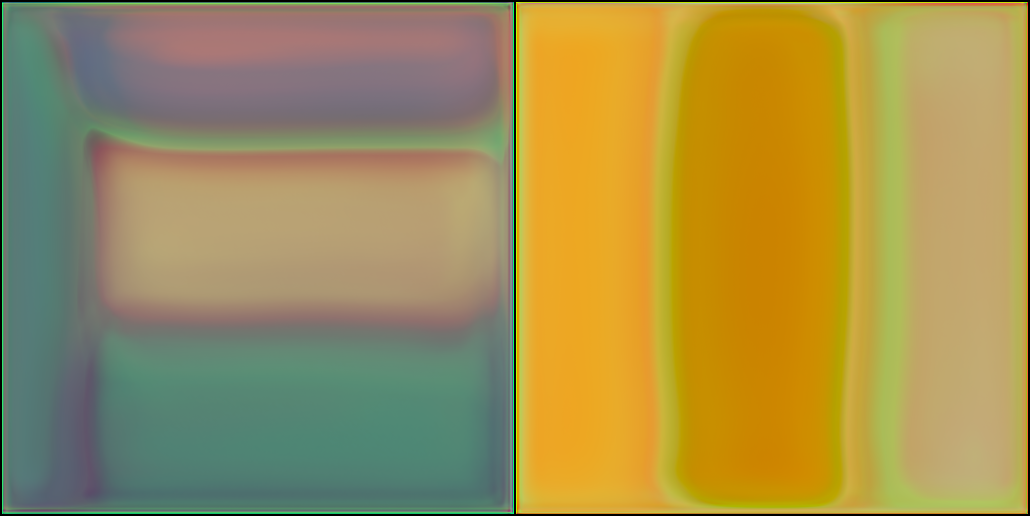
\includegraphics[width=1\textwidth]{figures/c7_impact/ue_1_1_still.png}
    \caption{Still from \textit{(un)stable equilibrium 1:1}.}
    \label{fig:c7:ue_still}
\end{figure}

The works were first shown in the exhibitions for the respective conferences ICCV and NeurIPS in 2019. 
At NeurIPS the works were shown in the AI Art Gallery, alongside where the work was presented as a workshop presentation at the NeurIPS Workshop for Creativity and Design. 
At ICCV the work was shown in the Computer Vision Art Gallery, where it won the Grand Prize in Computer Vision Art , an honour that is only shared between myself \citep{broad2019unstable}, Anna \citet{ridler2018mosaic} and Nouf \citet{aljowaysir2021salaf}.

The work was shown in a gallery setting in march 2020 in Geneva, Switzerland at One Gee in Fog, though unfortunately that exhibition had to be cut short after 2 days because of the imposition of the covid lockdown in Switzerland. 
In lockdown, I began producing prints of the works onto metal aluminium plates, which were extremely glossy and saturated. 
Initially I was selling these online through my own website. These works were later exhibited in the commercial London gallery \textit{the depot\_}, in their deput show titled \textit{the depot\_ digs} \citep{depot2021digs} (Figure \ref{fig:c7:depot_digs}), where I was also invited to give an artists talk in 2021.

\begin{figure}[!htb]
    \centering
    \captionsetup{justification=centering}
    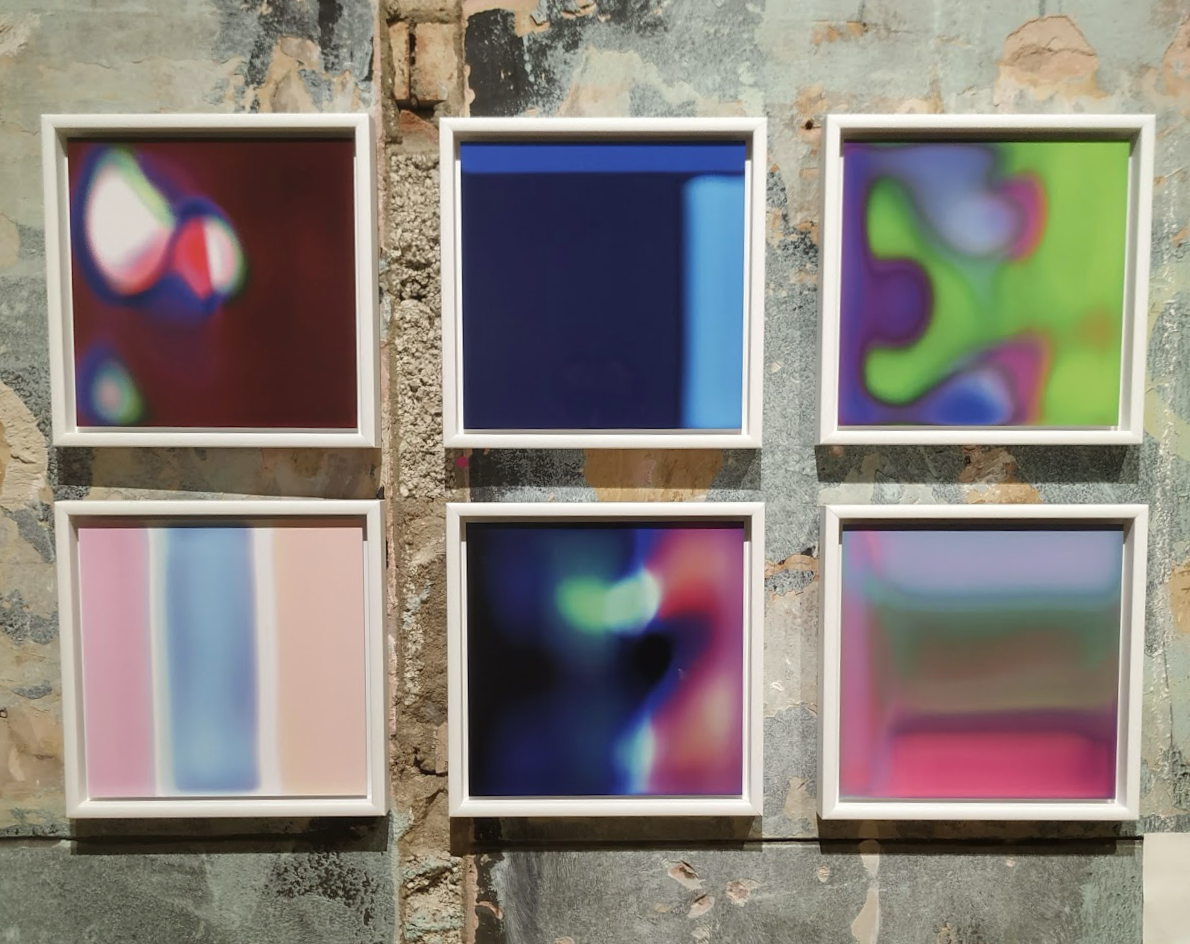
\includegraphics[width=1\textwidth]{figures/c7_impact/depot_cropped.png}
    \caption{Installation shot of \textit{(un)stable equilibrium} prints in \textit{the depot\_ digs} exhibition at the depot\_ gallery in London (2021).}
    \label{fig:c7:depot_digs}
\end{figure}

Following the covid pandemic, the work was later shown at FILE festival. 
File Festival is the premier digital arts festival in South America, where the work was installed in the Fiesp cultural centre in São Paolo (Figure \ref{fig:c7:file-festival}). 
Here, the work was presented as it’s originally intended incarnation as a lopping video piece.

\begin{figure}[!htb]
    \centering
    \captionsetup{justification=centering}
    \includegraphics[width=1\textwidth]{figures/c7_impact/FILE-festival.png}
    \caption{Installation shot of \textit{(un)stable equilibrium 1:1} at \textit{FILE Festival} in the Centro Cultural Fiesp, São Paolo (2022).}
    \label{fig:c7:file-festival}
\end{figure}

\section{Divergent fine-tuning}


Directly from the latter set of experiments described in Chapter 4, inverting the objective function, the series of artworks \textit{Being Foiled} (Figure \ref{fig:c7:being-foiled}), were produced using the model checkpoints after 500 iterations from the 512x512 StyleGAN FFHQ model. 

\begin{figure}[!htb]
    \centering
    \captionsetup{justification=centering}
    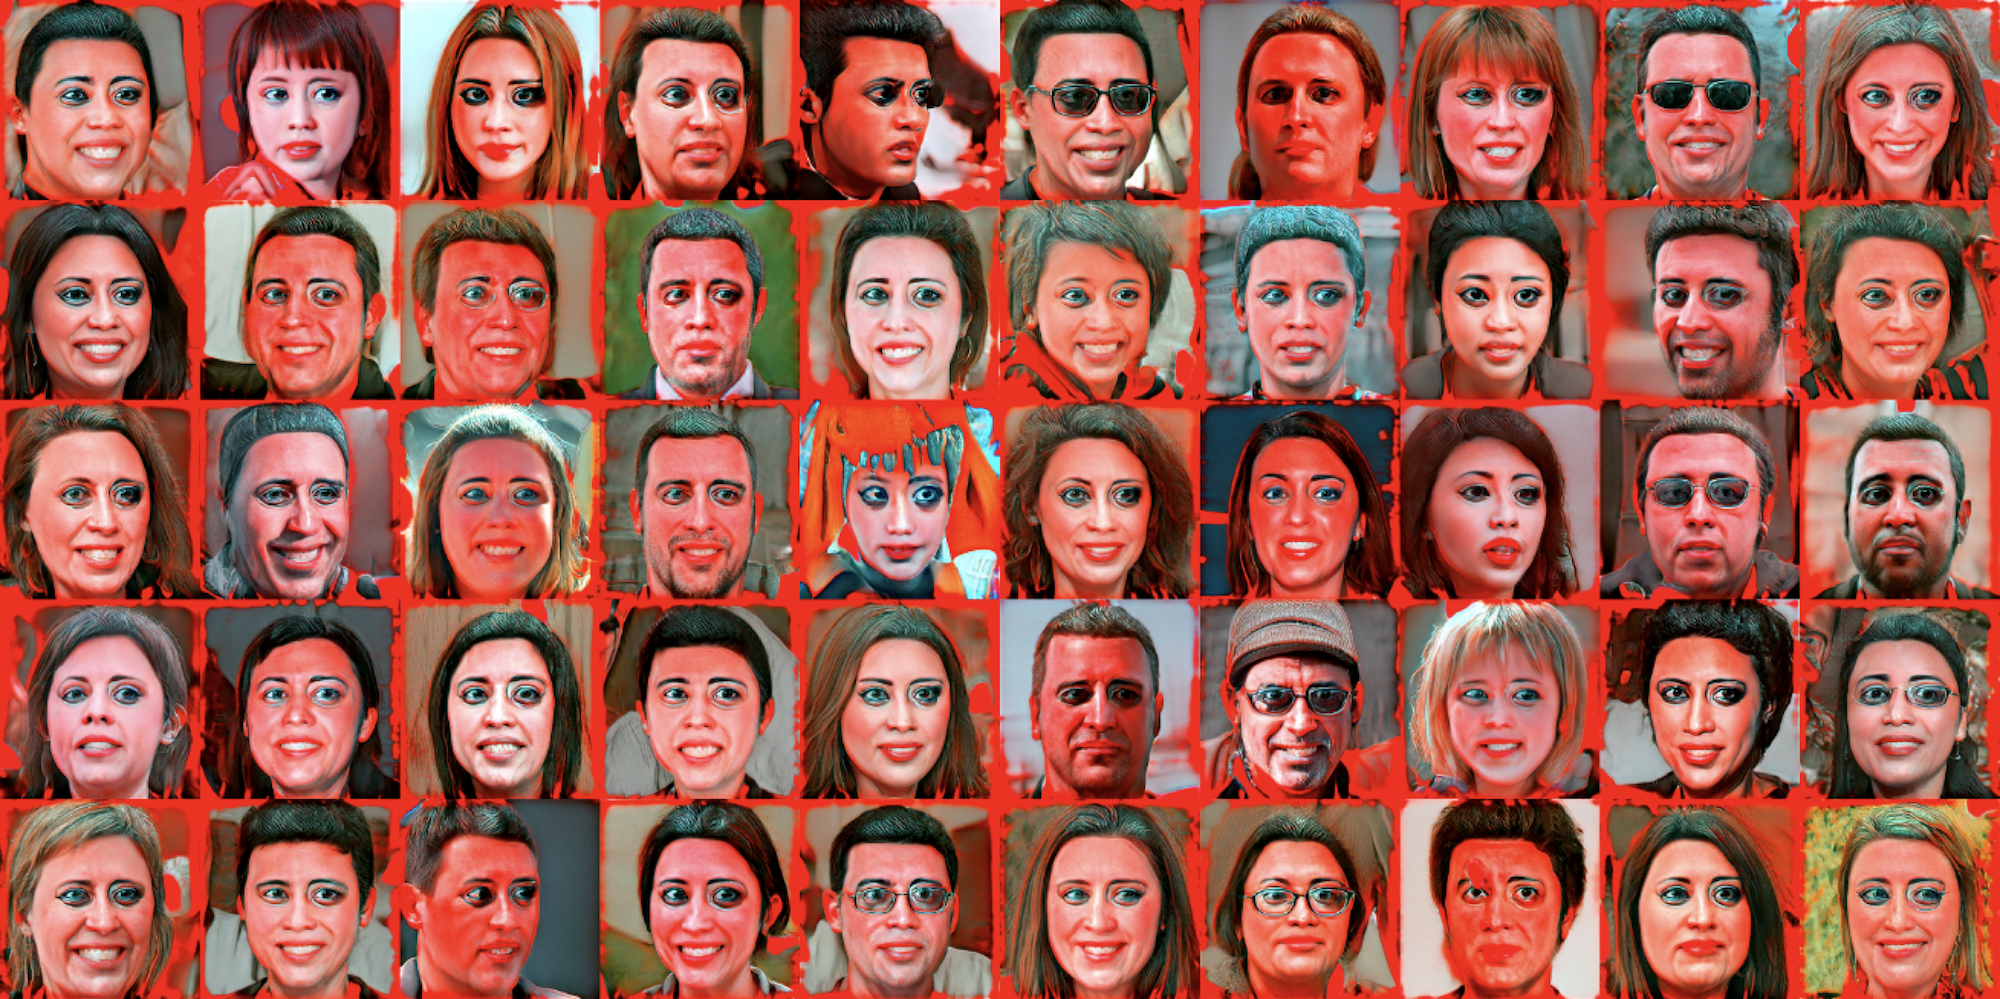
\includegraphics[width=1\textwidth]{figures/c7_impact/being-foiled.png}
    \caption{\textit{Being Foiled} (2020).}
    \label{fig:c7:being-foiled}
\end{figure}

The paper Amplifying the uncanny, that described the second set of experiments in Chapter \ref{ch:uncanny}, after being published in xCoAx was cited by \cite{berns2020bridging} in their paper ‘Bridging generative deep learning and computational creativity’. 
It was in this paper that they coined the term active divergence, in an original taxonomy with four categories: latent space search, cross-domain training, early stopping and rollbacks and loss hacking. 
Where the last category, loss hacking was describing the work described in chapter 4. 
I later went on the write an expanded survey and taxonomy of active divergence methods, in collaboration with Sebastian Berns and Simon Colton, which is covered in the next chapter.

Freezing the weights of the discriminator and using them for fine-tuning, as was used in both experiments in Chapter \ref{ch:uncanny}, was later also used in the \textit{freezing the discriminator} method \citep{mo2020freeze}, where only the lower layers of the discriminator model were frozen, and used to aide and assist in the fine-tuning step.
Investigating the representations of the frozen discriminator network after training was performed by \citet{porres2021discriminator} in his paper, discriminator synthesis, using the gradient methods popularised in the deep dream algorithm to visualise internal feature activations of the discriminator network.

The experiments described in chapter 4 were the first published descriptions of methods for performing divergent fine-tuning, which has since had many developments. 
The most notable being StyleGAN-NADA, which uses the CLIP network to fine-tune with auxiliary characteristics of another network \citep{gal2021stylegan}, in much the same fashion as the first experiment in chapter 4 was trying to describe. 
% The most notable other fine-tuning is human-guided reinforcement learning (RL-HF) \citep{ziegler2019fine}, which is used to considerable success in ChatGPT \. 
% These techniques along with other methods for performing divergent fine-tuning are described in more detail in Section [REF] of the following chapter.  

\section{Artworks made with network bending}

A number of artworks have been made with the network bending framework, by myself, and by others. 
This section will detail them in a (mostly) chronological order.

\subsection{\textit{Teratome}}

Early on in the experimental development of the network bending framework, I was hand-coding modifications to the neural network code and seeing the respective changes. 
These were simple mathematical formulations, like ablation $x*0$ and inversion $x-1$ of the feature maps. 
The most significant effect of these manipulations occurred in the first few layers of the generator. 
At first, I was doing these layer-wide, and later on, I was performing these to a random selection of the feature maps in a single layer. 

\begin{figure}[!htbp]
    \subfloat{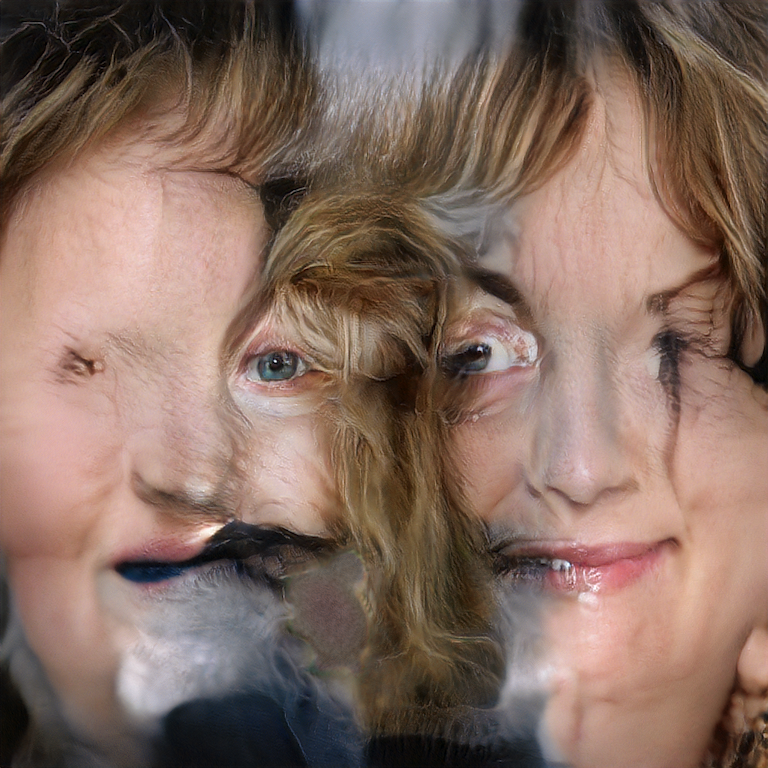
\includegraphics[width=.48\textwidth]{figures/c7_impact/teratome/1.png}}
    \hfill
    \subfloat{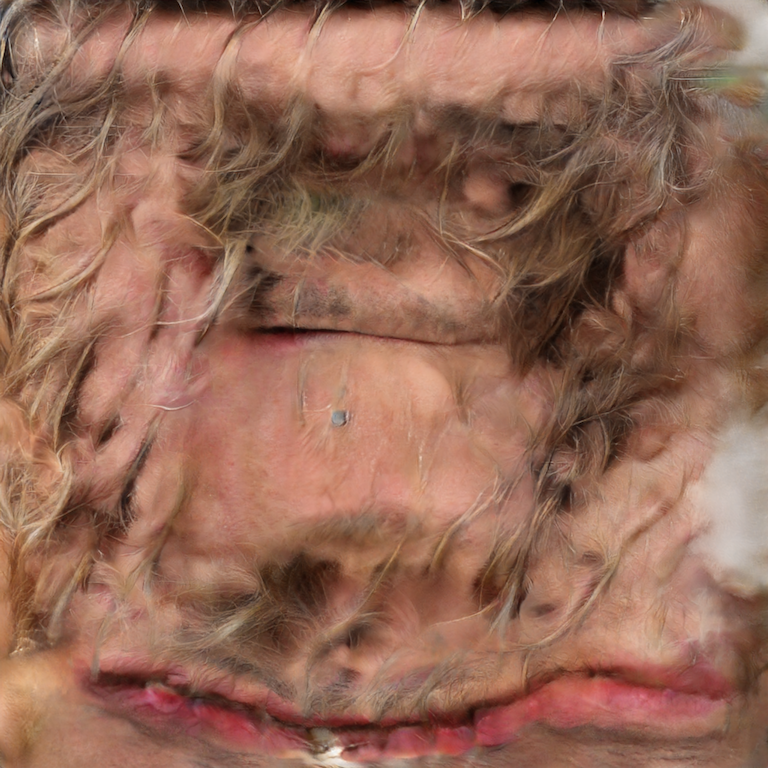
\includegraphics[width=.48\textwidth]{figures/c7_impact/teratome/2.png}}
    \hfill
    \subfloat{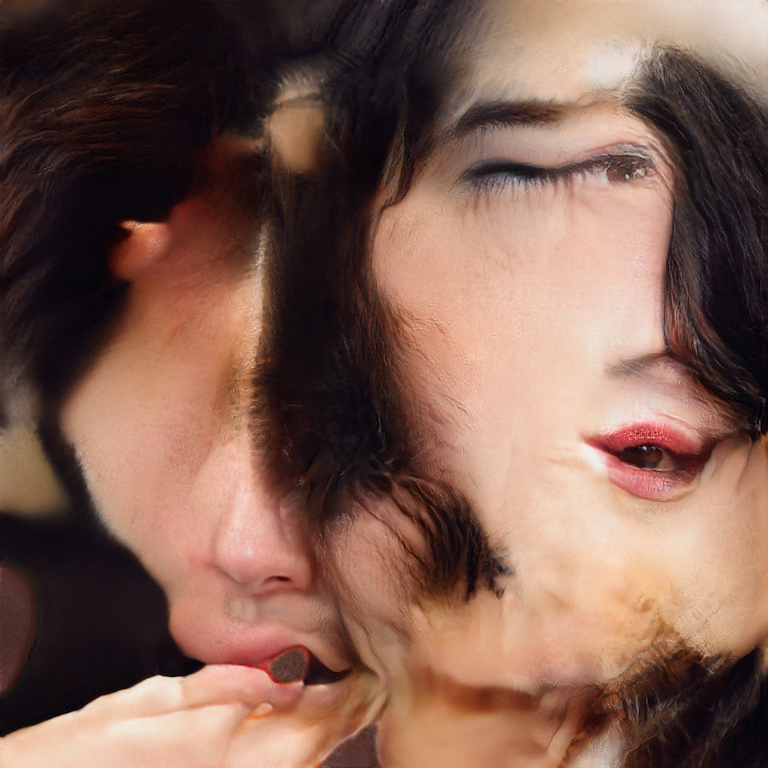
\includegraphics[width=.48\textwidth]{figures/c7_impact/teratome/3.png}}
    \hfill
    \subfloat{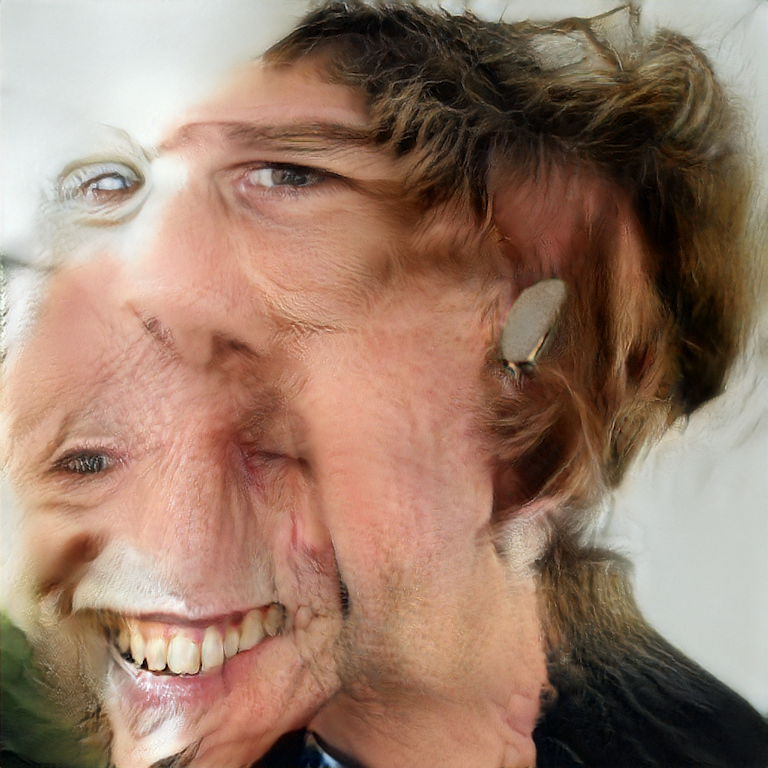
\includegraphics[width=.48\textwidth]{figures/c7_impact/teratome/4.png}}
    \caption{\textit{Teratome} (2020).}
    \label{fig:c7:teratome}
 \end{figure}

One of the things that struck me when examining the randomly selected manipulations of feature maps within a layer, was that 1 in 50 or 100 images, recognisable characteristics would be preserved in ways not seen in the other samples. 

For instance, eyes, mouth, would be in-tact in the generated results. This exploratory stage of work is what led to the intuition that groups of features, rather than the approach of examining individual features taken by the GAN Dissection work, would be important to allow for my semantically meaningful control and manipulation of the generated results. 

These early experimental images were first kept to myself. 
But In the autumn of 2020, some months after publishing the original network bending preprint on arxiv, I revisited them and hand-picked some of the most striking results as a series of artworks named \textit{Teratome} (Figure \ref{fig:c7:teratome}). 

The works from the series \textit{Teratome} were one of the jurors selected works in the NeurIPS AI Art Gallery in 2020 \citep{broad2020teratome} and the HCI-Art gallery at the CHI conference in 2022 \citep{perry2022art} . 
The documentation of which was later made into a subsequent book publication where the artworks also featured \textit{The State of the (CHI)Art} \citep{sturdee2023chiart}. 

\subsection{\textit{Disembodied gaze}}

Another artwork that was made during the development of the network bending framework was the work disembodied gaze. 
This was made shortly after I completed the work on the clustering algorithm and investigating the results. 
One of the clusters from the algorithm that had the clearest effect was the cluster in layer 5 that determined eyes. 
When ablated the cluster, the eyes disappear and the model fills in the gaps with skin. 
This alone was quite a surprising result. But when all the features but the eyes are ablated, things get a lot more surprising. 

\begin{figure}[!htbp]
    \subfloat[]{\label{subfig:eyes}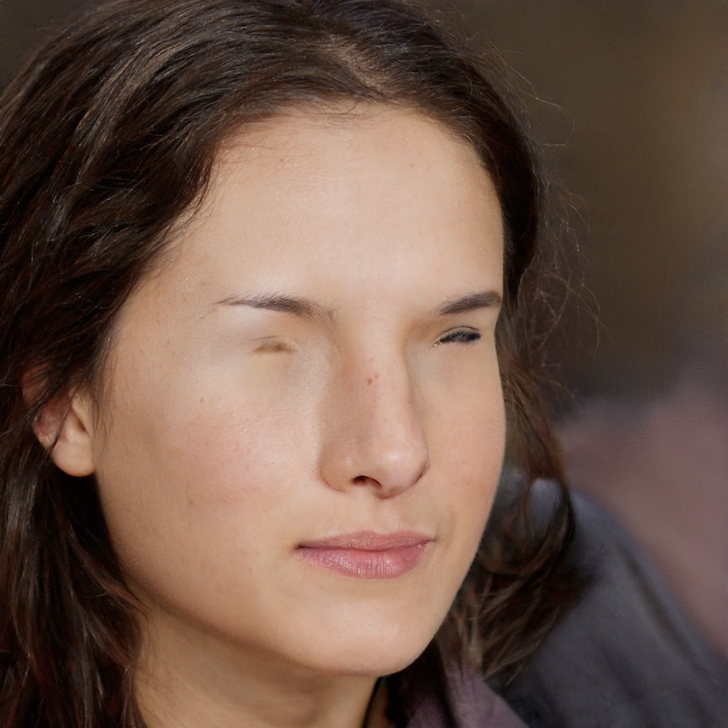
\includegraphics[width=.48\textwidth]{figures/c7_impact/eyes-off.png}}
    \hfill
    \subfloat[]{\label{subfig:no-eyes}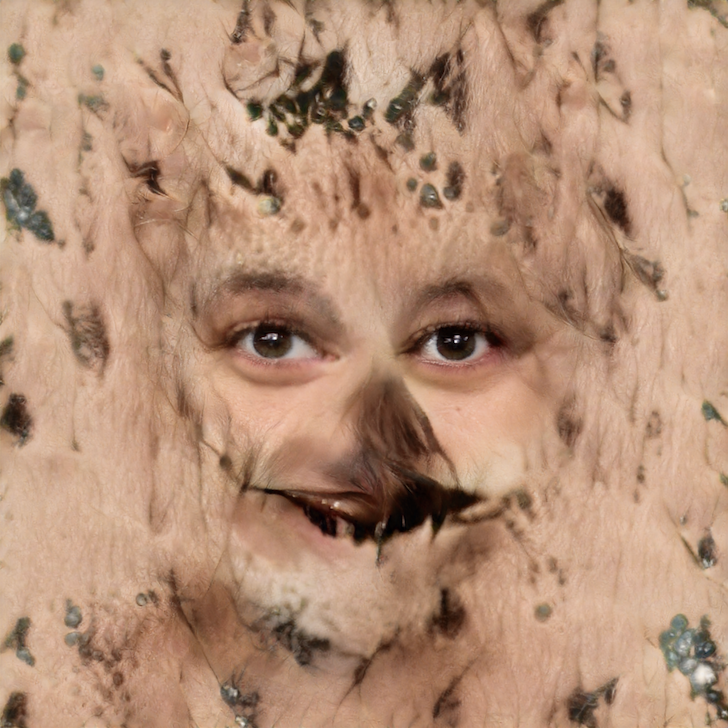
\includegraphics[width=.48\textwidth]{figures/c7_impact/eyes-on-face-off.png}}
    \hfill
    \caption{(a) Image generated using network bending with cluster controlling the generation of eyes ablated. (b) Image generated with network bending where all convolutional features apart from those that generate eyes are ablated.}
    \label{fig:c7:eyes-no-eyes}
 \end{figure}

I was struck by the bizarre textural regions that were filled in the background. 
The ghostly smile. 
I experimented with making a latent interpolation video with this model. StyleGAN latent space interpolations were very popular back in 2019-2020 time, and I personally was not that keen on them. 
They were quite a cheap trick to do with any newly trained styleGAN model and I found them quite nauseating. 
However with this intervention, I did not get the nauseating morphing in the same way. 
Though the identities were changing, so much of the recognisable characteristics were gone, leaving only the eyes as a fixed point in the video, contrasted with the stochastic nature of the textural background. 

After making an initial video at the standard square aspect ratio (1024x1024), ubiquitous for latent space interpolation videos at the time, I set about making a work that was bigger and at a more cinematic aspect ratio. 
I developed a network bending transformation layer that mirrored that extended the width of the activation maps by padding the sides of them with zeros. 
As all of these regions were already ablated in the network, these appear seamless in the generated result. 
This was not a feature that I shared publicly on the network bending git. It would probably not have the desired effect in all cases. 
It could use a lot of memory, and it was easy to break the code without entering the right input parameters.

\begin{figure}[!htb]
    \centering
    \captionsetup{justification=centering}
    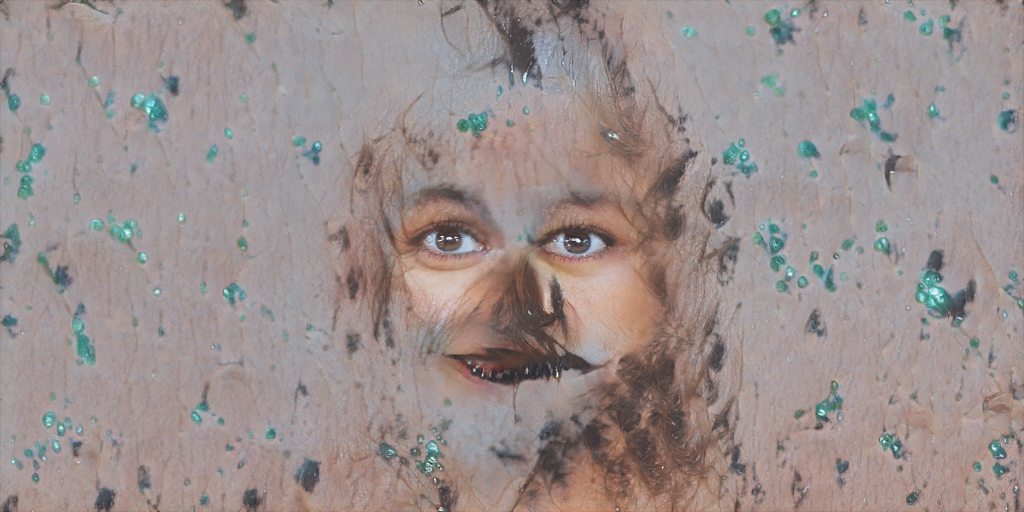
\includegraphics[width=1\textwidth]{figures/c7_impact/disembodied_gaze.png}
    \caption{Still from \textit{Disembodied Gaze} (2020).}
    \label{fig:c7:disembodied-gaze-wide}
\end{figure}

After some cropping and formatting of the video into a commonly used aspect ratio, and creating a seamlessly looping video 13 minutes in length, I created the video work Disembodied gaze \citep{broad2020disembodied}. 
This work was never exhibited as such, but I revisit it alot in artist talks. 
It is a good illustration of what is possible with network bending, and is a good demonstration of something that is unique to the approach, and would be near impossible to make any other way. 
The widening layer was also something I used later on in the \textit{Fragments of Self} work detailed in \S \ref{c6:subsubsec:fragments}.

\subsection{EP Artworks for \textit{0171}}

In the spring of 2020, I was approached by musicians from the band 0171, who were releasing a series of EPs that autumn. 
They had seen my work Being Foiled, and had been interested in using images from those series of some of the EP covers. 
They were keen to have images of themselves distorted in that way, though because the implementation of StyleGAN1 I had used for that model didn’t have an available projection model, it was not going to be straightforward to do that for them as I was occupied with finishing the network bending development. 
I did, however, inform them I was working on something new, which because I was using stylegan2 that had a projection implementation available, meant I could work with images from the band as a starting point, before projecting them into stylegan2 latent space and doing manipulation with them. 

They provided me with one of their press shots (Figure \ref{fig:c7:0171-press-shot})  that was to be used for their forthcoming PR-push. 
I cropped the respective faces of the two band members, and projected them into StyleGAN2 latent space, using the gradient method \citep{abdal2019image2stylegan} (Figure \ref{fig:c7:0171-crop-embed}).

\begin{figure}[!htb]
    \centering
    \captionsetup{justification=centering}
    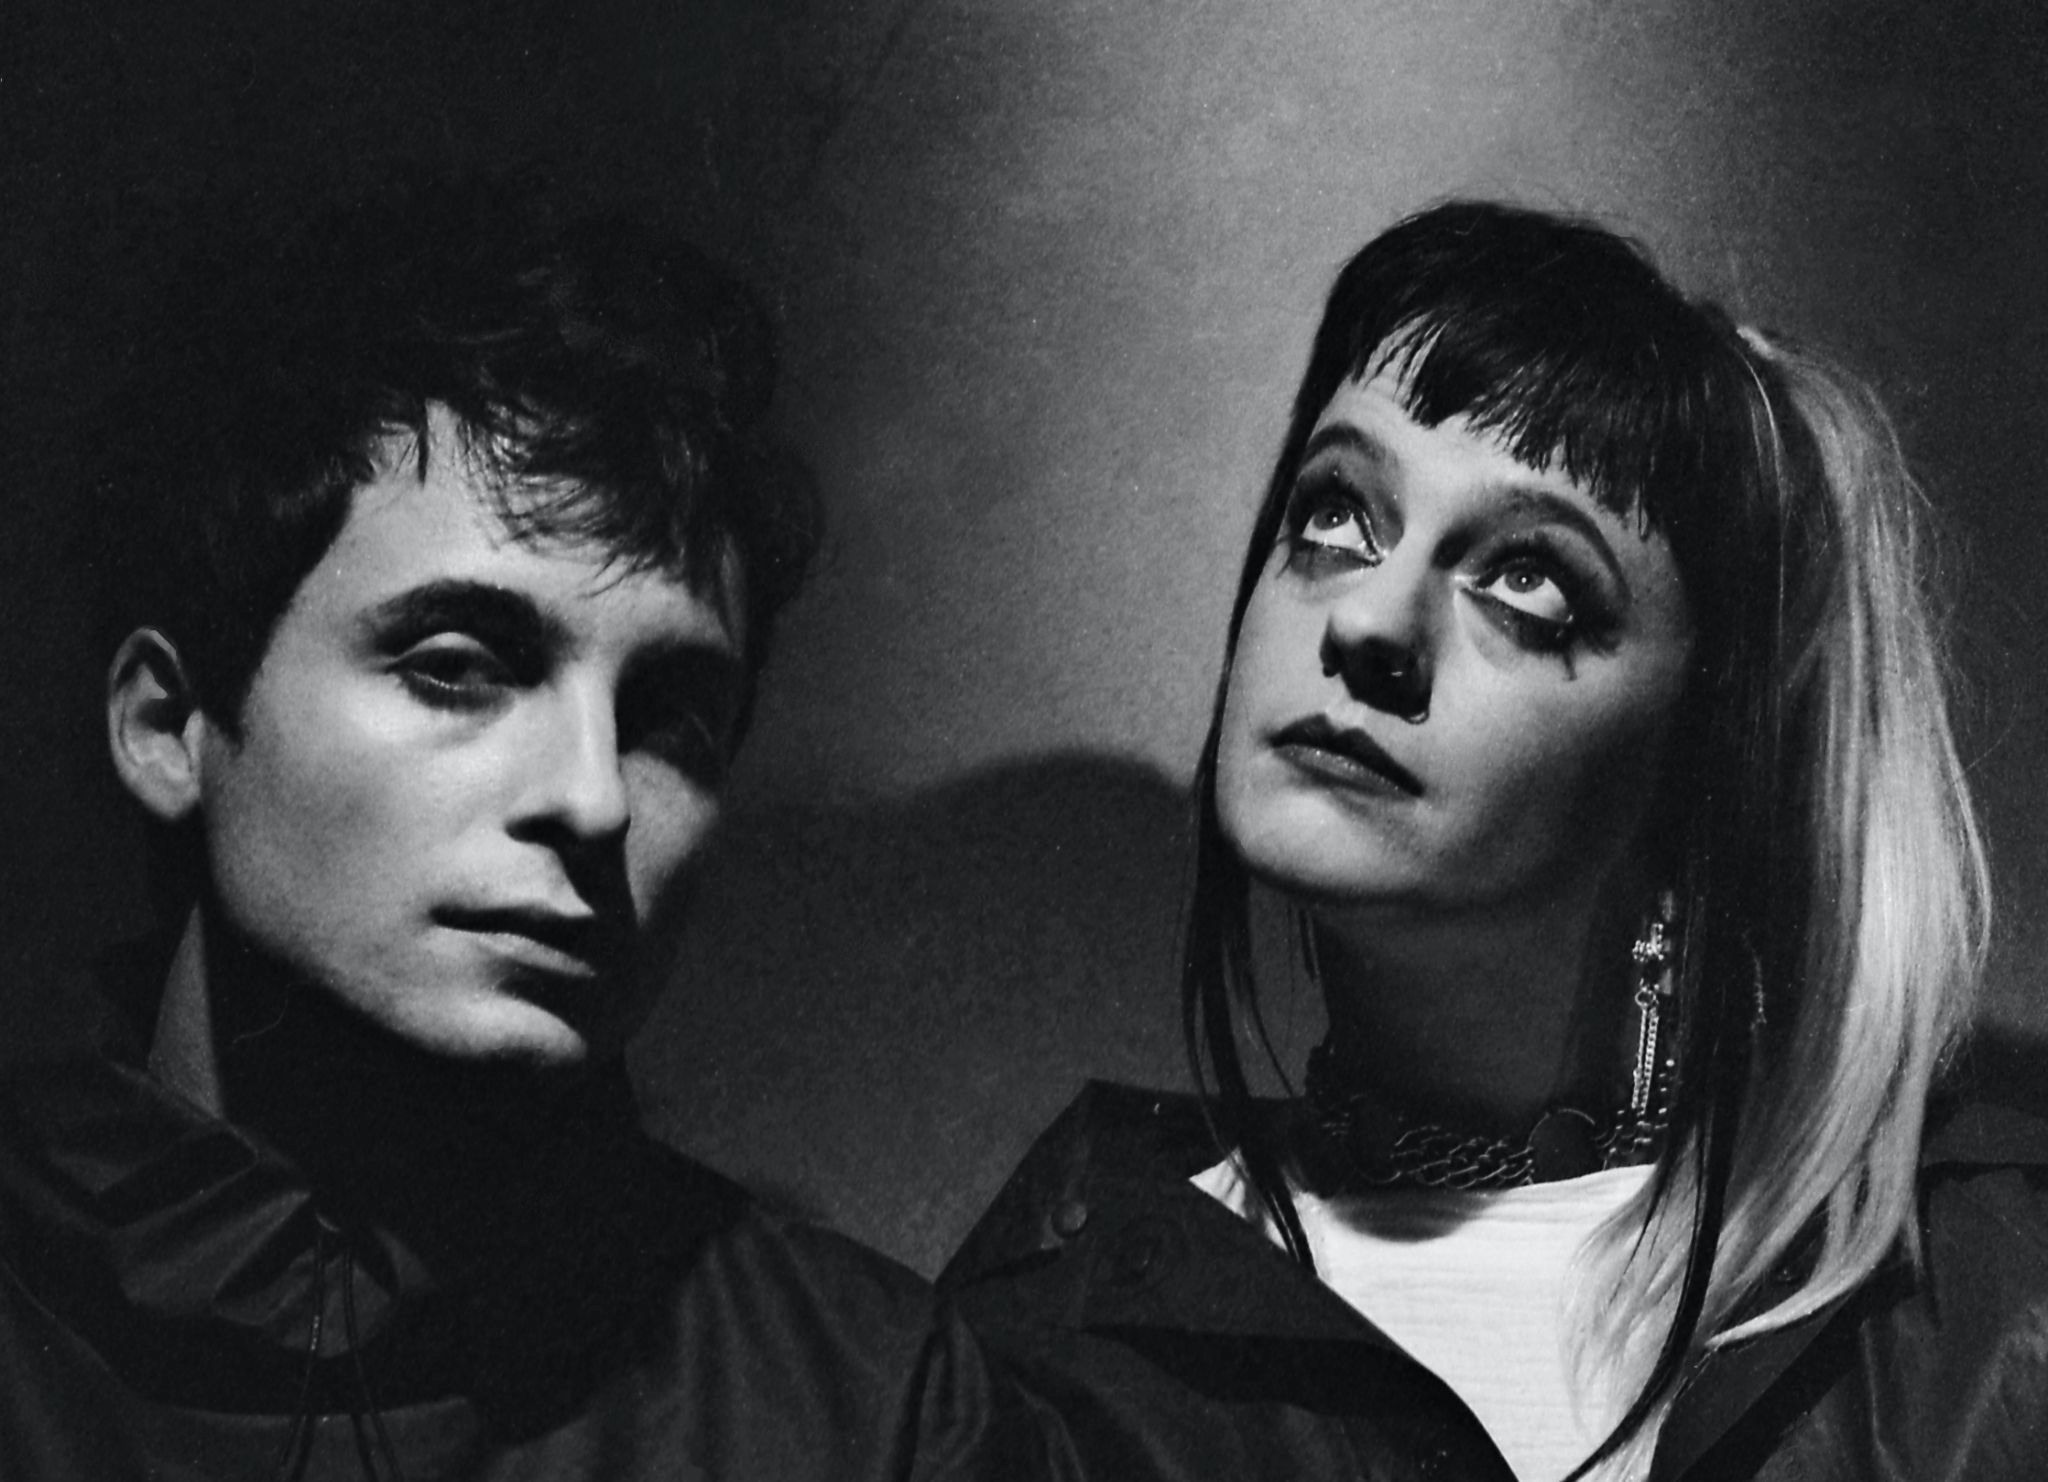
\includegraphics[width=1\textwidth]{figures/c7_impact/0171/press/0171-press-shot.png}
    \caption{0171 Press shot.}
    \label{fig:c7:0171-press-shot}
\end{figure}


\begin{figure}[!htbp]
    \subfloat[]{\label{subfig:joe-cropped}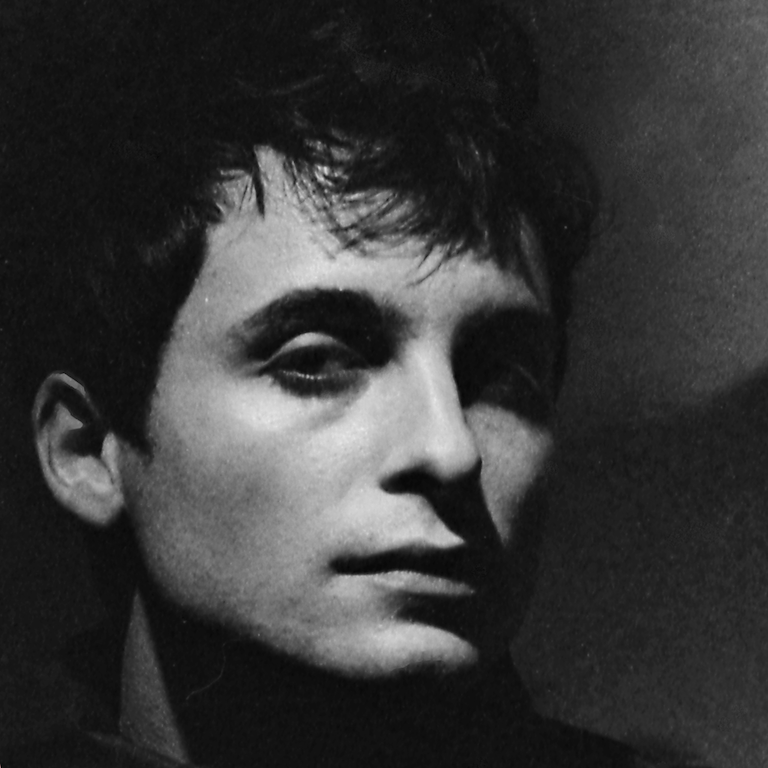
\includegraphics[width=.24\textwidth]{figures/c7_impact/0171/press/joe-cropped-press.png}}
    \hfill
    \subfloat[]{\label{subfig:joe-latent}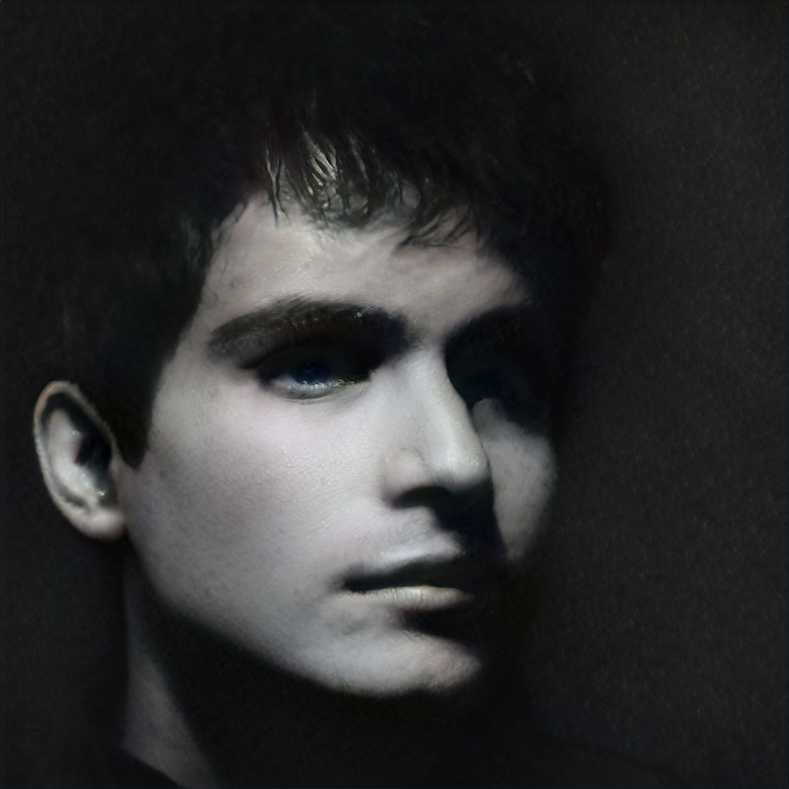
\includegraphics[width=.24\textwidth]{figures/c7_impact/0171/press/joe-cropped-style.png}}
    \hfill
    \subfloat[]{\label{subfig:georgie-cropped}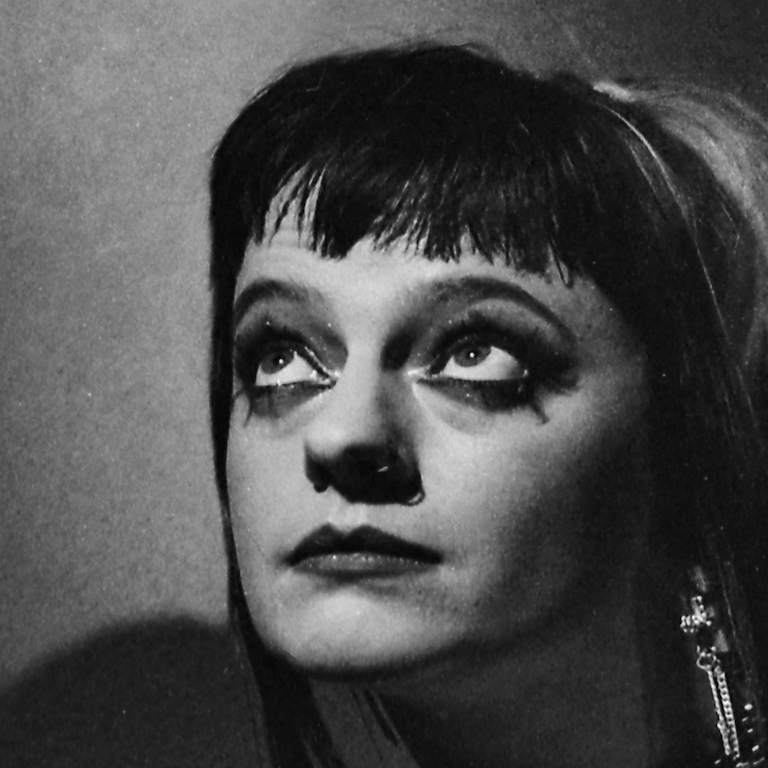
\includegraphics[width=.24\textwidth]{figures/c7_impact/0171/press/georgie-cropped-press.png}}
    \hfill
    \subfloat[]{\label{subfig:georgie-latent}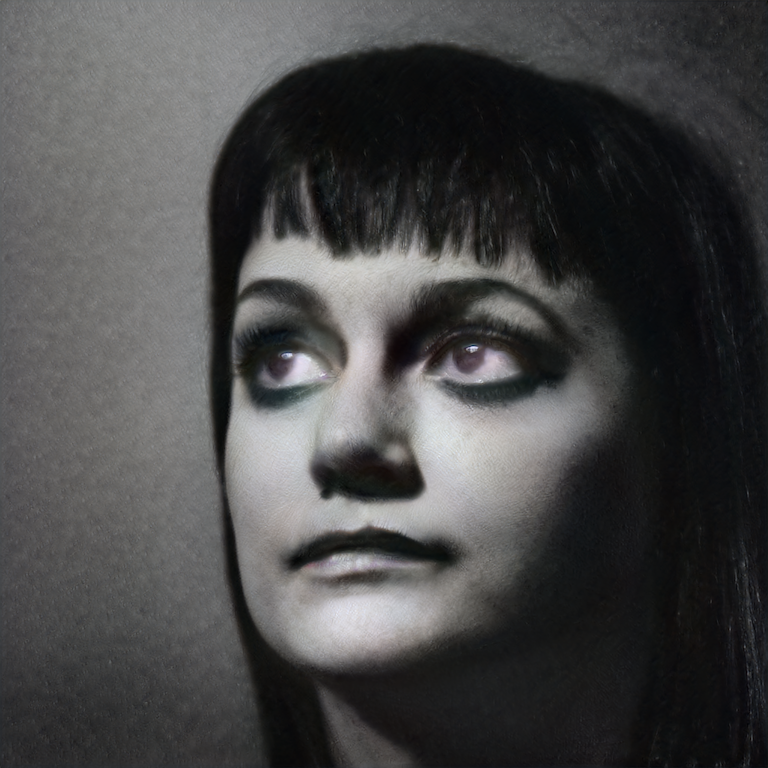
\includegraphics[width=.24\textwidth]{figures/c7_impact/0171/press/georgie-cropped-style.png}}
    \caption{Images of the individual band members cropped from the press shot (a,c) and their respective styleGAN2 projections (b,d). }
    \label{fig:c7:0171-crop-embed}
 \end{figure}


I took an exploratory approach to finding combinations of stochastic and layer wide transformations to the models, using this as an exercise to understand how transformations could be combined to produce more divergent and original images. 
I would keep the latent the same, alternating between the latents for the two respective band members, testing out different configurations of transformations parameters. 
I would generate 20 images using one setting, and there would always be variation in the images because of the stochastic layer transformations used. 
There would be more significant variation if these were used in the earlier layers of the GAN, or the percentage of random features distorted with a transformation was increased.

I would experiment intuitively with different configurations of transformations. 
If the set of results did not have much interesting variation I would boost the random threshold for features applied, and if it had too much I would tone these down. 
If one configuration produced a particularly fruitful set of results, I would generate more using the same parameters -- i.e. 100 or 1000. 
After experimenting like this for several days I selected my favourite samples and shared those with the band.

\begin{figure}[!htbp]
    \subfloat[]{\label{subfig:joe-h-1}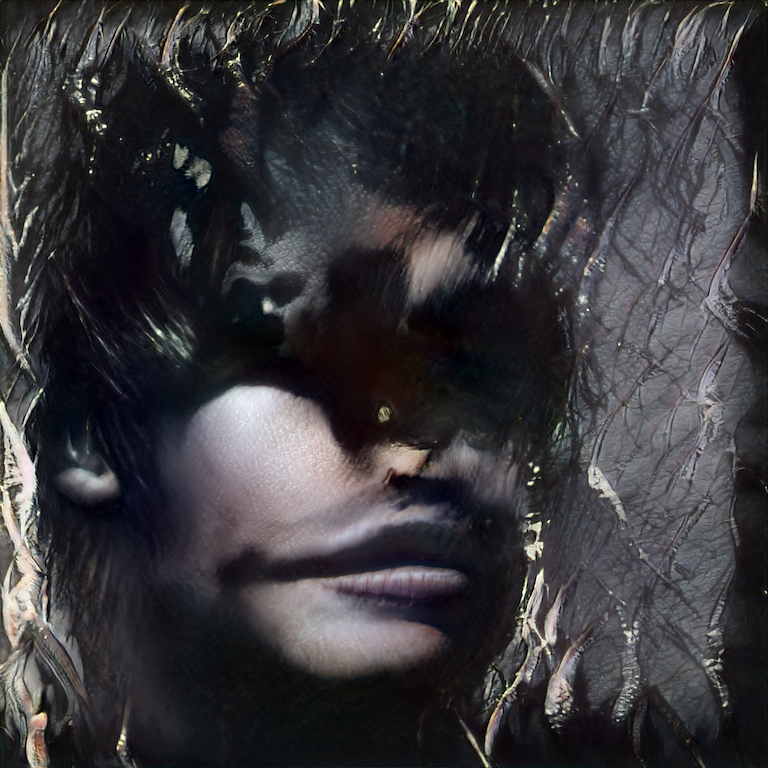
\includegraphics[width=.32\textwidth]{figures/c7_impact/0171/haunted/joe-1.png}}
    \hfill
    \subfloat[]{\label{subfig:joe-h-2}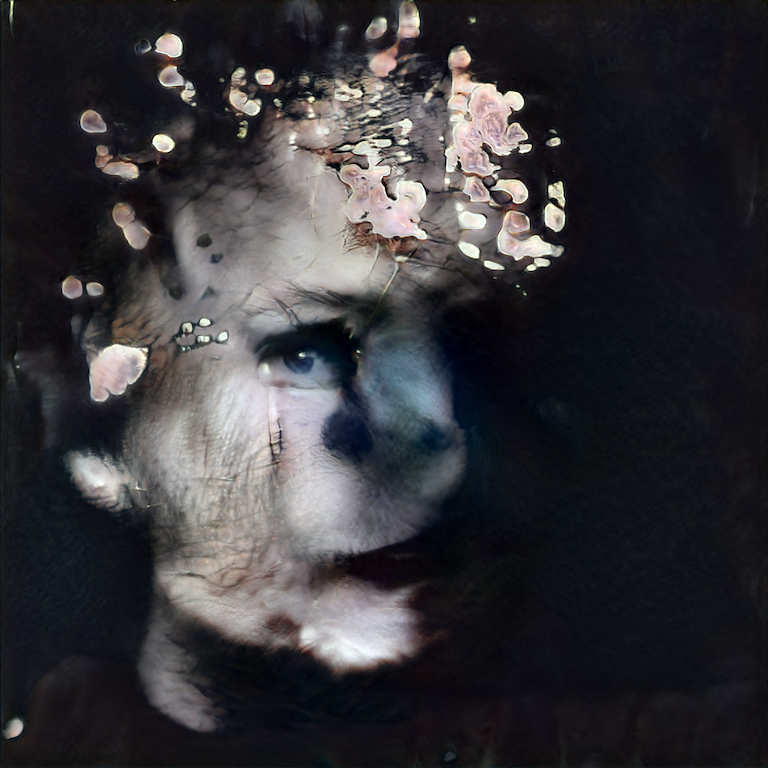
\includegraphics[width=.32\textwidth]{figures/c7_impact/0171/haunted/joe-2.png}}
    \hfill
    \subfloat[]{\label{subfig:joe-h-3}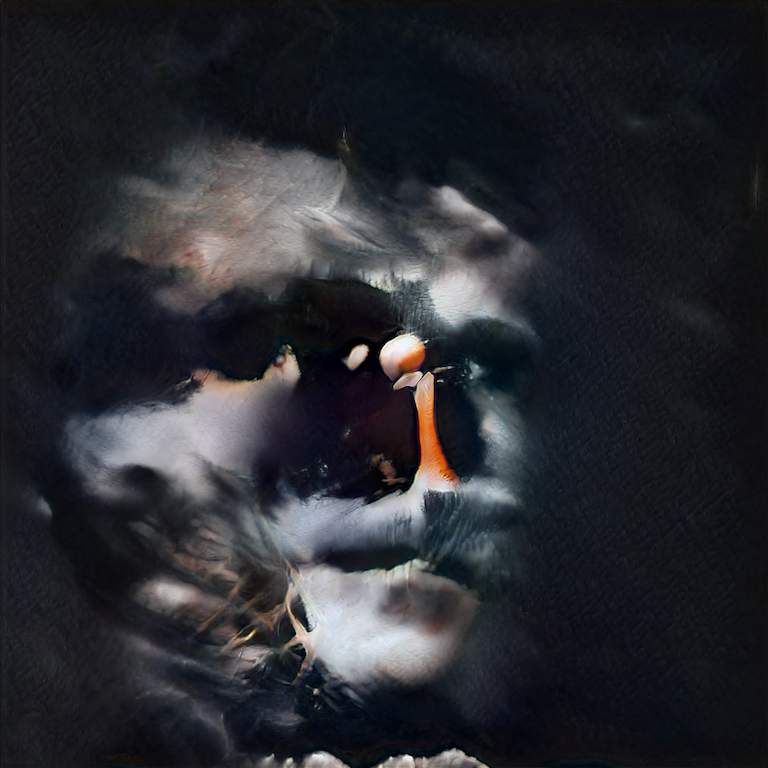
\includegraphics[width=.32\textwidth]{figures/c7_impact/0171/haunted/joe-3.png}}
    \hfill
    \subfloat[]{\label{subfig:georgie-h-1}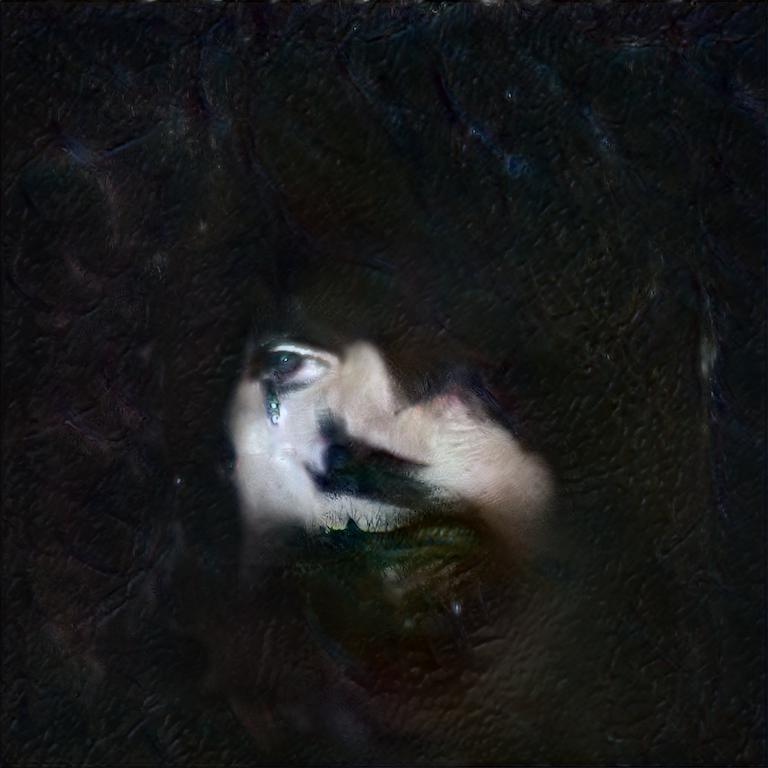
\includegraphics[width=.32\textwidth]{figures/c7_impact/0171/haunted/georgie-1.png}}
    \hfill
    \subfloat[]{\label{subfig:georgie-h-2}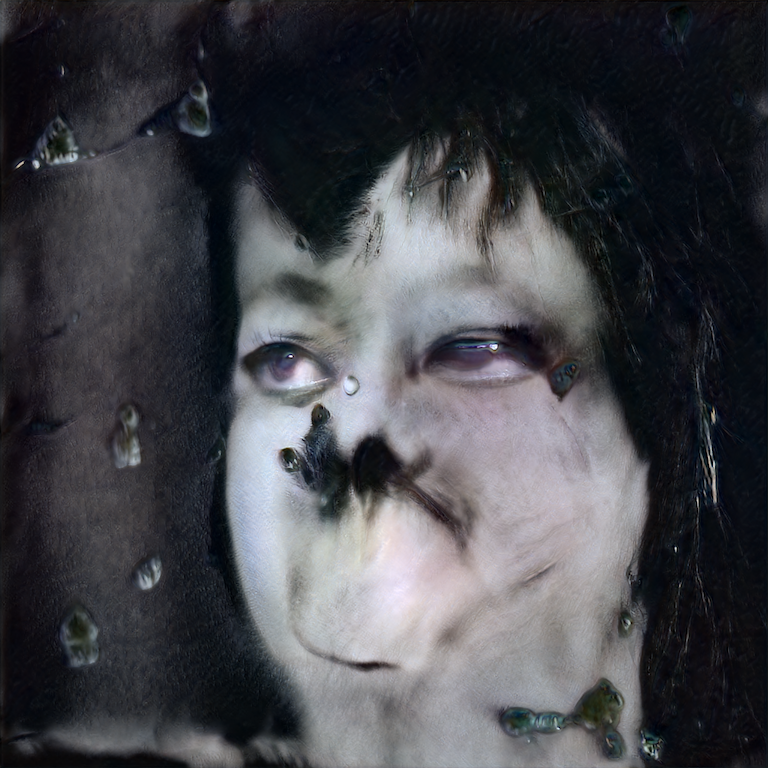
\includegraphics[width=.32\textwidth]{figures/c7_impact/0171/haunted/georgie-2.png}}
    \hfill
    \subfloat[]{\label{subfig:georgi-h-3}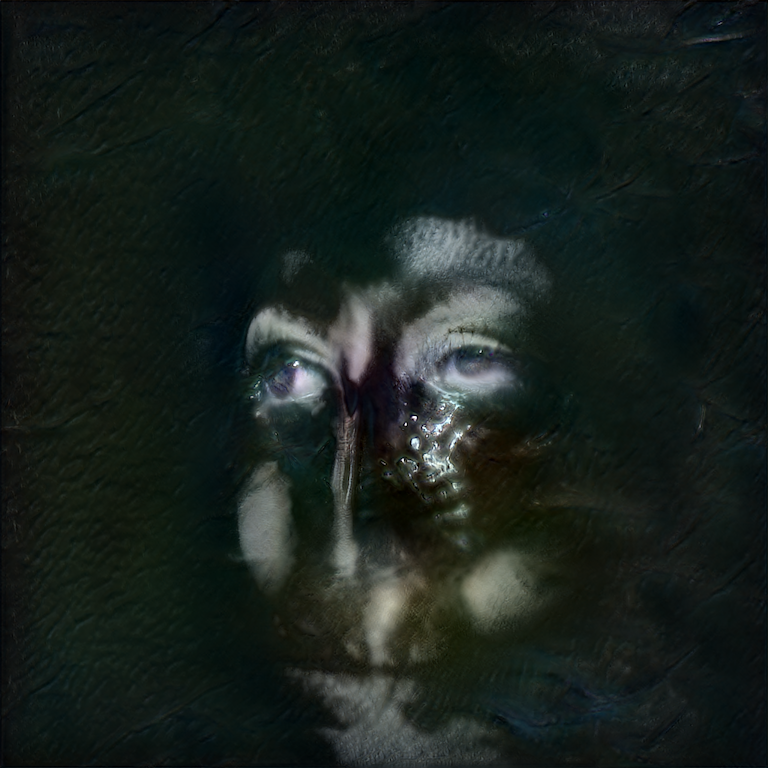
\includegraphics[width=.32\textwidth]{figures/c7_impact/0171/haunted/georgie-3.png}}
    \hfill
    \caption{(a-c) images generated using network bending techniques applied to the latent \ref{subfig:joe-latent}, (d-f) images generated using network bending techniques applied to the latent \ref{subfig:georgie-latent}.}
    \label{fig:c7:0171-haunted}
 \end{figure}

I shared these original works with the band, and while they were very impressed with the result, they were not quite in-line with the desired aesthetic for a synth-pop band (Figure \ref{fig:c7:0171-haunted}). 
The original images were sourced from a dark, black and white film photograph, which had been deliberately distorted with scratches and other physical interventions made to the film. 
As the latents were conditioned on this image, the dark, gothic look was persistent in the results, and accentuated by the facial distortions present. 
I advised them that if they wanted something more colourful and pop friendly, then using a different more colourful image of themselves as the starting point would work better.
They provided me with headshots taken in front of a colourful painting, which we then used for the project. 

I began repeating the process described earlier with the previous latent vectors of the band members. 
Trying out the same latents that produced interesting results with the previous latents, and adapting them to work better with these latents. 
Not all transform configuration settings that worked with the previous latents worked well with these, without some tweaking. 
Showing that there was a clear contingency between how well different latents and transform parameter configurations would work well.
In addition, based on feedback from the band members that the distorted but recognisable faces were also not aligned with the appearance the band were trying to give off, I amped up the level of distortion so that the distortion was so great that they appeared more abstract than before. 
This time, the band members themselves were more involved in the process. I would experiment with transformation parameters, select some of my personal favourites, show these to the band who would tell me what they liked and disliked and that would inform further experimentation. 
We ended up with 10 pictures (?), 5 for each band member, and they selected their favourite 10 of these for the 4 EP and single releases (Figure \ref{fig:c7:0171-EP}). 

\begin{figure}[!htbp]
    \subfloat[]{\label{subfig:ep1}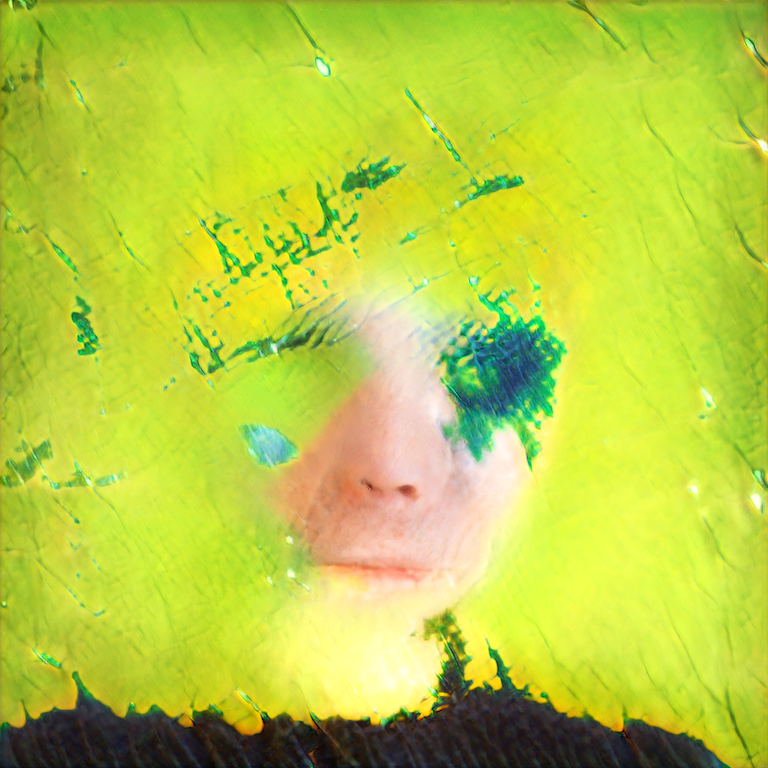
\includegraphics[width=.48\textwidth]{figures/c7_impact/0171/ep/automatic.png}}
    \hfill
    \subfloat[]{\label{subfig:ep2}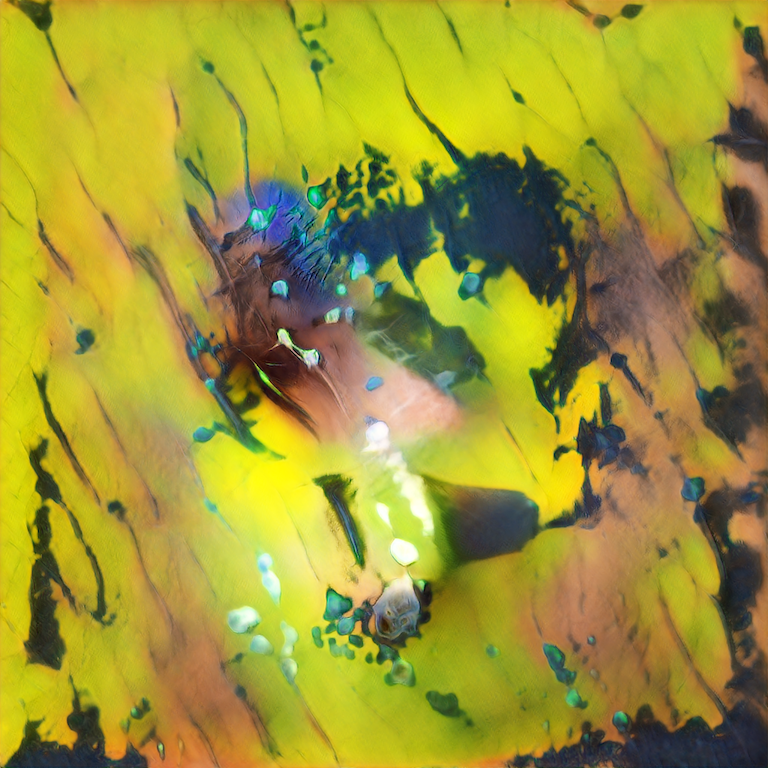
\includegraphics[width=.48\textwidth]{figures/c7_impact/0171/ep/follow.png}}
    \hfill
    \subfloat[]{\label{subfig:ep3}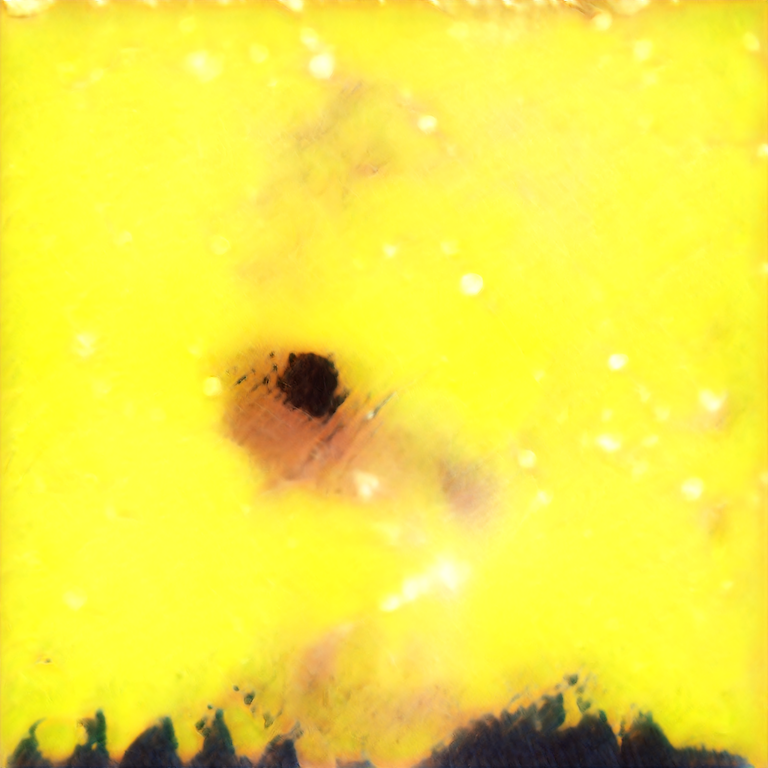
\includegraphics[width=.48\textwidth]{figures/c7_impact/0171/ep/photograph.png}}
    \hfill
    \subfloat[]{\label{subfig:dp4}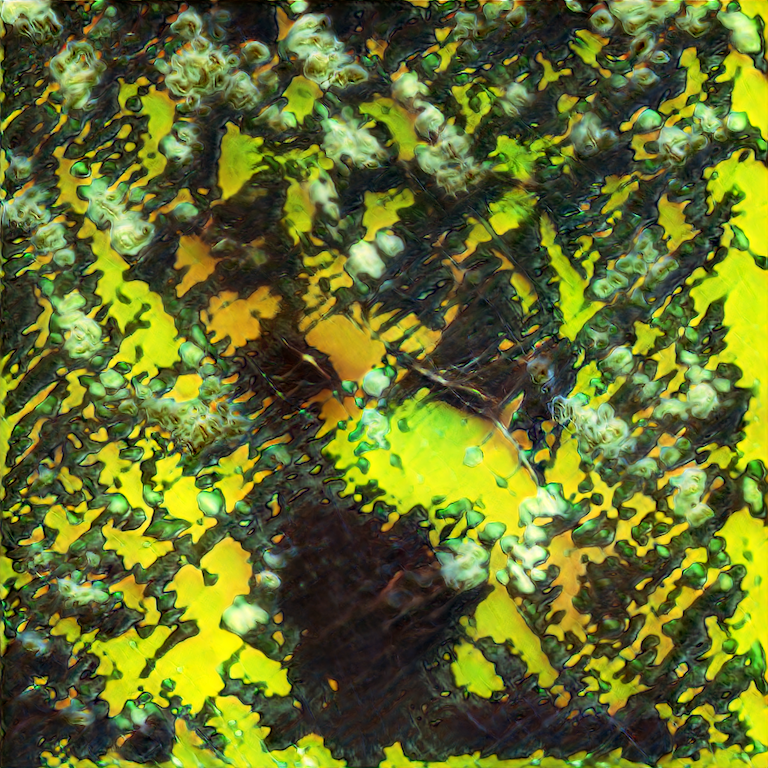
\includegraphics[width=.48\textwidth]{figures/c7_impact/0171/ep/change-nothing.png}}
    \caption{EP and single artworks created for the band 0171. (a) Artwork for single \textit{Automatic}. (b) Artwork for the single \textit{Follow}. (c) Artwork for the single \textit{Photograph}. (d) Artwork for the EP compilation \textit{Change Nothing}.}
    \label{fig:c7:0171-EP}
 \end{figure}

Working on this series of artworks as the network bending framework was in development was fortunate in its timing (this all happened prior to me getting long-covid), as it served as a useful case study early on in the development of this framework in a real world application, and later being detailed in the original EvoMUSART paper \citep{broad2021network} 
The EP artworks can be seen on any streaming service or digital music platform, and the earlier images (in Figure \ref{fig:c7:0171-haunted}) were later used to produce the NFT artworks Haunted Variations \citep{broad2021haunted1,broad2021haunted2}. 

\subsection{\textit{Fragments of self}}
\label{c6:subsubsec:fragments}

After producing some striking visuals with the transformations of the band members, I would have been remiss if I were not to have performed the same transformations to myself. 
I took a self portrait photograph of myself from a holiday in Croatia and projected that into StyleGAN2 latent space. 

\textbf{Figure:Selfie + crop + video}

I took some of the random transformation configurations that were used for the final 0171 EP artworks and tried them on myself. But these were rendered largely unrecognisable. 
I therefore tuned down some of the random parameters and made some other minor adjustments until the results were more clearly recognisable as bearing some similarities in likeness to myself.

\textbf{Figure:Samples}

None of these images, by themselves, were starkly close to my own recognition. 
The level of distortion was still quite high.
Individually the images were quite amusing, and provided quite a lot of entertainment value looking through them. 
As I was navigating through them on the ubuntu image viewer, by pressing the right and left keys, if I held these keys and scroll quickly through the images, as if they were in motion, the resemblance to myself was much stronger. I ended up stitching together 1000 of these randomly generated images into a looping video approx 10 seconds long, and making a short video piece that was shared on social media. 
Like the work disembodied gaze, this was not exhibited anywhere, but is something I share regularly in artist talks as it is a good, and amusing illustration of the possibilities offered by the framework I have generated. 
It was not until I was invited to participate in the exhibition Reflections in the water curated by Luba Elliot on the digital art gallery platform Feral File, that this line of enquiry had any major impact. 

I was unsure of what I was going to exhibit in this show, but I was given the curators notes from Luba several months in advance for the exhibition opening: 

\begin{quote}
``Working with AI art sometimes feels like gazing into a pond of water — we are not sure what we will get as a reflection. [...] Looking into a still pond, we see a clear, gently blurred version of ourselves staring back at us, while turbulent waters return mere rippled echoes of our shape. These changing reflections of ourselves are similar to images generated from data, which can be hyper realistic depictions of the original, or images that are surreal and barely recognizable, as flaws and errors creep in. [...]

GAN technologies have improved much over the years [...] present[ing] a surprising challenge to AI art practitioners—what to do now that perfect realism is within reach? [... W]orking with AI has the potential to change too, as the technology becomes more predictable and controllable, rendering blurry reflections, distorted forms and uncertain outcomes a thing of the past.'' \citep{elliot2021reflections}.
\end{quote}

I was very inspired by some of the passages in these exhibition notes, and wanted to make an artwork that best fit with the theme. 
The description of seeing a distorted representation of ourselves reflected in the results of AI generated images rang particularly true, reflecting on the experiment with the selfies that I detailed here.

I took some headshot photographs and started projecting them into the StyleGAN latent space and experimenting with network bending. 
One headshot in particular, taken against an overcast skyline on a sunny day, had quite an interesting effect when projected. 
The background became oversaturated off white, and was quite uniform. Network bending transformations like ablation and inversion made the face disappear into the uniform background. 
Applying these transformations to this particular latent gave a resemblance to the description of gazing at a reflection of the self in distorted waters, and I set about creating an animated sequence that was as closely aligned to that visual metaphor as I could.

Sequencing frames where transformations are applied at random between each made for very chaotic viewing, which I wanted to dampen somewhat. 
I wanted to manipulations to more closely follow the description of a reflection in a turbulent body of water, so I set about creating a more coherent temporal way of interpolating between random selections of features in a layer to manipulate. 
Here I opted to use perlin noise. If each filter in a layer of 512 could be thought of as one pixel in a row of pixels, and the value between 0 and 1 could be used as the parameter to determine if a feature gets ablated, using a threshold that could be tweaked by hand. 
If we had a row that would be one set of transformations to be ran. 
If we generated a 2D image, that could be interpreted as a sequence of transformation parameters, where each row represented one time step.
% CHECK DESKTOP MACHINE TO SEE THE PROPER DETAILS ON THIS.

In the end, I renderd a 4/5d tensor of perlin noise, ( CHECK details on this). T
his gave me the sequence of transformations that would smoothly change from one frame to the next. 
After tweaking with the parameters, I ended up with the right ratio of features ablated in each time step. 
I wanted at each image, most of my face to be missing from the rendering. 
A fragment of my face, which could be recognisable overall but any individual frame it would be unrecognisable. 

\textbf{FIGURE: Fragments of Self final}

The final work was titled \textit{Fragments of Self}. 
At the time I could not explain why I was so drawn to these images of fragmented versions of myself. 
This was the first major artwork I had made during my recovery from long-covid, and on reflection, during this period of chronic illness, I did not feel like a whole person. 
The constant barrage of new symptoms, constantly changing ailments left me with the feeling of being a fragment of oneself for a long time.

\subsection{Jen Sykes' \textit{Field of View} and \textit{The Offing}}

Jennifer Sykes is an artist, designer and lecturer based in Glasgow, Scotland. 
She has used network bending in the production of several artworks. Building on a prior work, Places You’ve Never Been (cite), which used an archive of digitised film slides, that were captured from her family's migration from Canada to England, and used that to train a generative model. 

In Fields of View (CITE), Sykes uses the clustering algorithm of network bending to “change our interpretation to isolate ‘semantic groupings’ that include only the sky or only the mountains of a specific narrative?”. 
Exploring the personal archive of family images of migration, network bending is used to produce a selective generation of aspects of those archival images. 
Sykes likens this process to “historic in-camera editing techniques of cameraless film-making” as the manipulation is happening to the features present within a dataset, with no new footage being needed.

In The Offing (CITE), Sykes uses the same dataset and network bending transformations to manipulate landscape images. 
Here, clusters have been isolated that relate to the sky and the land, and these images are rotated in an animated sequence. 
The work produces “ a narrative stitched together through layers of the horizon; where land meets sea”. 
A region of space colloquially referred to as the offing. 

\subsection{Derrick Schultz's \textit{You Are Here}}

Derrick Schultz is an artist, designer and educator based in Brooklyn, New York. Scultz teaches on the Interactive Telecommunications Program at the The New York University Tisch School of the Arts, and online under his own range of popular online courses for making AI art called Artificial Images. 
Schultz has used Network Bending in a number of his own artworks, and has even produced tutorials showing others how to use it (CITE). 

To create the video work You Are Here (CITE), Schultz combined network bending with other machine based forms of image manipulation and processing to produce original results divergent from any original training data (a process I describe as Chaining models in more detail in the following chapter). 
Scultz uses a custom StyleGAN model trained on illustrations of flowers and renders from latents interpolation. 
While rendering Schultz applied network bending transformations to add rotation to the image and have that processing in real-time. 
That image is then fed into an image translation model (BigBiGAN) to get a different, further divergent image. 
The final machine learning step schultz uses is SuperSlowMo (CITE) to stretch to duration for the sequence to 1000x the original length,

\textbf{FIGURE: STORY BOARD COMPARISON}

For Schutlz, using this esoteric and complex chain of computational models was a way to separate himself from other AI artists who were training styleGAN models on similar datasets, and the create results that you couldnt produce with one single GAN model designed to imitate a specific dataset. 
Scultz likens this process of switching outputs between ml models to Sloans theory of flip-flopping (CITE), which is a practice in design where works are created from switching from digital to physical space.

\subsection{Hans Brouwer's \textit{Ouroboromorphism}}

Ouroboromorphism (CITE) is an audiovisual work made by Hans Brouwer, an artist and researcher working towards his Masters degree at the Delft University of Technology. 
This work was created with and part of a broader investigation into developing audio-reactive StyleGAN latent interpolations (CITE). 

Using a custom StyleGAN model, trained on abstract imagery (presumably to minimise recognisable representations so more visual bandwidth can be used for communicating audio feature information).
 Brouwer uses audio features to manipulate the latent vector codes for real time generation. 
 In addition he uses network bending transformations to add an additional level of control of manipulating the visuals in response to audio, that would be possible with latent vector manipulation alone, which allows for “increasing the musical information that can be conveyed in a given period of time.”. 

Network bending was used in response to two sets of audio features that are recognised.
If Kicks (sound resembling a kick-drum) are found to be in the audio sequence, a zooming effect will be made to correspond to that sequence in time. If a snare (sound resembling a snare-drum) is made, then a horizontal translation is made of the visuals. 
Brouwer also achieves a larger resolution and 2:1 aspect ratio by mirroring the activation maps in the earlier layer of the gan so that all of the generations are doubled with then onwards, in a similar manner to how I achieved the wider aspect ratio with Disembodied gaze and fragments of self. 

In addition to network bending, Brouwer adopted model rewriting (Cite) as another active divergence method that can be used to manipulate the visual representations. 
I discuss these method in more detail in the following chapter which surveys active divergence methods.

\section{Technical impact of Network Bending}

The network bending paper has gone on to have influenced further technical development of direct manipulation techniques, generative model architecture design and be integrated into many user interface designs, all detailed in this section.

 \subsection{Alias-Free GAN (aka StyleGAN3)}

 Alias-free GAN (later renamed StyleGAN3) by Kerras et al. (2021) was NVIDIA corporations successor to their flagship StyleGAN1 and 2 neural networks. 
 The alias-free GAN approach, was designed from the ground up to be fully equivariant to transformations of their internal representations (aka network bending). 
 This architecture can produce internal features that are equivariant to either two kinds of transformation, translation or rotation. 
 Having a network architecture that was better suited to manipulation of the internal representations of the model has, in their words, “pave[d] the way for generative models better suited for video and animation.” \citep{karras2021alias}.

 One of the artefacts revealed when network bending was performed on StyleGAN2 models was the ‘texture sticking’ effect, that can be seen when animating a transformation, such as a translation or rotation, where the fine-details are stuck to specific pixel coordinates. 
 The authors attributed the texture sticking to “unintentional positional references made to intermediate layers from the borders of the image, per-pixel noise inputs and aliasing between layers”. 
 The traditional network architecture “ha[ve] the means and motivation to amplify even the smallest amounts of aliasing and combine it over multiple scales to build a basis for texture motifs that are fixed in screen coordinate space” \citep{karras2021alias}.
 Reflecting on this, they make a major overhaul to the convolutional framework used in the generative model and replace the convolutional layers in the generator with pointwise convolutional layers.

 \textbf{FIGURE: SG3 rotation video screenshot}

 The alias-free GAN paper cites our original network bending paper from EvoMUSART, and it is clear, from the direction of the research and it’s evaluation in technical and public facing demo’s that network bending has informed and the direction of research in this advancement of the technical development work of the architecture and the evaluation of those improvements and how that is communicated publicly. 

StyleGAN3 was and largely still is the state-of-the-art in fidelity and controllability of GAN architectures. 
While this went on to be superseded in terms of fidelity and flexibility of image generation by diffusion based models, particularly, latent diffusion, at the time of writing StyleGAN3 is still one of the SOTA models for feed-forward image generation, with network bending was core to its inspiration and development. 

\subsection{Interfaces Developed for Network Bending}

Building an interface was something that I had originally planned as follow on work from the original network bending paper in 2020. 
Now while this was derailed by the pandemic. In-person user studies were not possible (and building one that worked online would have required a complete re-architecture of the codebase), and because of suffering from long-covid, my ability to complete work on that scale, or even learn new skills and coding frameworks was severely hampered. 
In-line with the UKRIs guidance to PhD students to “adapt their research plan in response to restrictions to the pandemic to finish their work in a timely manner” I gave up on that idea and found an alternate focus for my PhD that did not require me to build, test and evaluate a user interface. 

Whilst I did not make a user interface for network bending myself. 
In the intervening period, between completing the experimental work and writing up the thesis many others have done exactly that. 
This subsection will detail all of the efforts to date for interfaces for network bending.

\subsubsection{StyleGAN3 Visualiser}

In the release of the StyleGAN3 codebase on github, NVIDIA corporation built and provided a user interface for interactively generating samples, visualising internal feature representations, and applying the x-y translation and rotation transformations. 

\textbf{FIGURE: SG3 visualiser screncap}


These translations are only applied layer wide, but the code is configured such that animations of these transformations being applied with linearly changing parameters can be applied. 

\subsubsection{Autolume}

In the AutoLume-live system (Kraasch \& Pasquier 2022) network bending is one several features integrated into a real-time GAN-based VJing system. 
The latent vectors are determined by musical features amplitude, pitch and onset strength. 
These audio features create latent trajectories for the animation created with the GAN. 
A MIDI-based interface is developed to allow the user to improvise and adjust this generative process in realtime, with network bending transformations being one of the manipulations that can be made. 

\textbf{FIGURE: Autolume screenshot}

\subsubsection{StyleGAN Canvas}

StyleGAN-Canvas is a mixed-intiative interface (Zhang 2023), combining image-to-image translation with rendering perfomed by styleGAN3. 
A custom encoder was trained to perform image to latent realtime encoding, allowing users to take webcam or other input images and use that as the starting point for GAN rendering. 
Parameters for controlling network bending transformations:  erosion, dilation, scalar-multiplication, x-y translations, rotation, and scaling. 
The clustering algorithm described in the previous chapter has also been implemented and clusters for StyleGAN3 models were calculated and integrated into the interface.

\textbf{Figure: Jaspers thingy screenshot}

\subsubsection{Other Network Bending Interfaces}

Talk about Nao Tuki's and Alex Rose Chalmers WIP Interfaces.

\section{Further advancements of Network bending}

\subsection{Network Bending DDSP}

The first extension of network bending was undertaken by Yee-king and McCallum (2020, 2021). 
In this work, they took the Differential Digital Signal Processing model (DDSP from Google Magenta, which is a neural network for audio synthesis and manipulation for tasks such as timbre transfer. 
he DDSP model takes frequency and amplitude values and it outputs 101 control values for an oscillator and noise filter parameters. 
In the network bending DDSP framework, network bending transformations are applied to the three layers in the neural network where all of the features are combined. 
There are four different types of transformation in this work: ablate, invert and binary threshold have been kept from the work described in the last chapter.
 In addition Yee-king and McCallum implemented an oscillate transformation that performs a sin wave transformation based on the frequency and the depth of the layer in the network. 

\subsection{PANDA}

TBC

\subsection{Network Bending gradient descent}

TBC

\subsection{Network Bending diffusion models}

TBC

\section{Conclusion}

This chapter has detailed the impact the experimental work in my PhD has had, in both the cultural and technical sectors. T
his includes detailing the artworks made by myself, other practitioners and the work done to extend and build interfaces to interact with the work I have developed. 
In particular, the network bending framework has been the work that has been most adopted by others. 
In all these cases, network bending has been adopted to allow for further generative possibilities that were available with traditional GAN training. 
Referring back to the title of this thesis \textit{Expanding the generative space}, it is this piece of work that has most successfully had an impact in that regard. 

The common goal of all of the experiments in chapters 3, 4 and 5 were to explicitly and actively divergence from the training dataset, rather than imitate it. 
Increasing the possibility space of what can be generated using neural networks. 
During the period of this PhD many others were working on achieving the same goal but by relating different means to the methods I developed. 
The next chapter is a survey of these methods, and includes a taxonomy giving an overview of all published methods and the key technical differences between methods given by myself and others. 
